%%%%%%%%%%%%%%%%%%%%%%%%%%%%%%%%%%%%%%%%%
% Programming/Coding Assignment
% LaTeX Template
%
% This template has been downloaded from:
% http://www.latextemplates.com
%
% Original author:
% Ted Pavlic (http://www.tedpavlic.com)
%
% Note:
% The \lipsum[#] commands throughout this template generate dummy text
% to fill the template out. These commands should all be removed when 
% writing assignment content.
%
%
%%%%%%%%%%%%%%%%%%%%%%%%%%%%%%%%%%%%%%%%%

%----------------------------------------------------------------------------------------
%	PACKAGES AND OTHER DOCUMENT CONFIGURATIONS
%----------------------------------------------------------------------------------------

\documentclass{article}

\usepackage{fancyhdr} % Required for custom headers
\usepackage{lastpage} % Required to determine the last page for the footer
\usepackage{extramarks} % Required for headers and footers
\usepackage[usenames,dvipsnames]{color} % Required for custom colors
\usepackage{graphicx} % Required to insert images
\usepackage{listings} % Required for insertion of code
\usepackage{courier} % Required for the courier font
\usepackage{lipsum} % Used for inserting dummy 'Lorem ipsum' text into the template
\usepackage{url}
\usepackage{amsmath}
\usepackage[shortlabels]{enumitem} 
\usepackage[T1]{fontenc}

% Margins
\topmargin=-0.45in
\evensidemargin=0in
\oddsidemargin=0in
\textwidth=6.5in
\textheight=9.0in
\headsep=0.25in

\linespread{1.1} % Line spacing

% Set up the header and footer
\pagestyle{fancy}
\lhead{\hmwkClass} % Top left header
\chead{(\hmwkClassInstructor\ \hmwkClassTime)} % Top center head
\rhead{\firstxmark} % Top right header
\lfoot{\lastxmark} % Bottom left footer
\cfoot{} % Bottom center footer
\rfoot{Page\ \thepage\ of\ \protect\pageref{LastPage}} % Bottom right footer
\renewcommand\headrulewidth{0.4pt} % Size of the header rule
\renewcommand\footrulewidth{0.4pt} % Size of the footer rule

\setlength\parindent{0pt} % Removes all indentation from paragraphs

%----------------------------------------------------------------------------------------
%	CODE INCLUSION CONFIGURATION
%----------------------------------------------------------------------------------------

\definecolor{MyDarkGreen}{rgb}{0.0,0.4,0.0} % This is the color used for comments
\lstloadlanguages{Python} % Load Python syntax for listings, for a list of other languages supported see: ftp://ftp.tex.ac.uk/tex-archive/macros/latex/contrib/listings/listings.pdf
\lstset{language=Haskell, 
        frame=single, 
        basicstyle=\small\ttfamily, % Use small true type font
        keywordstyle=[1]\color{Blue}\bf, % Python functions bold and blue
        keywordstyle=[2]\color{Purple}, % Python function arguments purple
        keywordstyle=[3]\color{Blue}\underbar, % Custom functions underlined and blue
        identifierstyle=, % Nothing special about identifiers                                         
        commentstyle=\usefont{T1}{pcr}{m}{sl}\color{MyDarkGreen}\small, % Comments small dark green courier font
        stringstyle=\color{Purple}, % Strings are purple
        showstringspaces=false, % Don't put marks in string spaces
        tabsize=4, % 5 spaces per tab
        %
        % Put standard Python functions not included in the default language here
        %morekeywords={rand},
        %
        % Put Python function parameters here
        %morekeywords=[2]{on, off, interp},
        %
        % Put user defined functions here
        %morekeywords=[3]{test},
       	%
        morecomment=[l][\color{Blue}]{...}, % Line continuation (...) like blue comment
        numbers=left, % Line numbers on left
        firstnumber=1, % Line numbers start with line 1
        numberstyle=\tiny\color{Blue}, % Line numbers are blue and small
        stepnumber=5 % Line numbers go in steps of 5
}

% Creates a new command to include a python script, the first parameter is the filename of the script (without .pl), the second parameter is the caption
\newcommand{\pythonscript}[2]{
\begin{itemize}
\item[]\lstinputlisting[caption=#2,label=#1]{#1.py}
\end{itemize}
}

%----------------------------------------------------------------------------------------
%	DOCUMENT STRUCTURE COMMANDS
%	Skip this unless you know what you're doing
%----------------------------------------------------------------------------------------

% Header and footer for when a page split occurs within a problem environment
\newcommand{\enterProblemHeader}[1]{
\nobreak\extramarks{#1}{#1 continued on next page\ldots}\nobreak
\nobreak\extramarks{#1 (continued)}{#1 continued on next page\ldots}\nobreak
}

% Header and footer for when a page split occurs between problem environments
\newcommand{\exitProblemHeader}[1]{
\nobreak\extramarks{#1 (continued)}{#1 continued on next page\ldots}\nobreak
\nobreak\extramarks{#1}{}\nobreak
}

\setcounter{secnumdepth}{0} % Removes default section numbers
\newcounter{homeworkProblemCounter} % Creates a counter to keep track of the number of problems

\newcommand{\homeworkProblemName}{}
\newenvironment{homeworkProblem}[1][Problem \arabic{homeworkProblemCounter}]{ % Makes a new environment called homeworkProblem which takes 1 argument (custom name) but the default is "Problem #"
\stepcounter{homeworkProblemCounter} % Increase counter for number of problems
\renewcommand{\homeworkProblemName}{#1} % Assign \homeworkProblemName the name of the problem
\section{\homeworkProblemName} % Make a section in the document with the custom problem count
\enterProblemHeader{\homeworkProblemName} % Header and footer within the environment
}{
\exitProblemHeader{\homeworkProblemName} % Header and footer after the environment
}

\newcommand{\problemAnswer}[1]{ % Defines the problem answer command with the content as the only argument
\noindent\framebox[\columnwidth][c]{\begin{minipage}{0.98\columnwidth}#1\end{minipage}} % Makes the box around the problem answer and puts the content inside
}

\newcommand{\homeworkSectionName}{}
\newenvironment{homeworkSection}[1]{ % New environment for sections within homework problems, takes 1 argument - the name of the section
\renewcommand{\homeworkSectionName}{#1} % Assign \homeworkSectionName to the name of the section from the environment argument
\subsection{\homeworkSectionName} % Make a subsection with the custom name of the subsection
\enterProblemHeader{\homeworkProblemName\ [\homeworkSectionName]} % Header and footer within the environment
}{
\enterProblemHeader{\homeworkProblemName} % Header and footer after the environment
}

%----------------------------------------------------------------------------------------
%	NAME AND CLASS SECTION
%----------------------------------------------------------------------------------------

\newcommand{\hmwkTitle}{Programming Project 2013\ \#1} % Assignment title
\newcommand{\hmwkDueDate}{Friday,\ May\ 24,\ 2013} % Due date
\newcommand{\hmwkClass}{COMP90053} % Course/class
\newcommand{\hmwkClassTime}{} % Class/lecture time
\newcommand{\hmwkClassInstructor}{Program Analysis and Transformation} % Teacher/lecturer
\newcommand{\hmwkAuthorName}{Diana Barreto, Ivan P. Valarezo} % Your name


%----------------------------------------------------------------------------------------
%	TITLE PAGE
%----------------------------------------------------------------------------------------

\title{
\vspace{2in}
\textmd{\textbf{\hmwkClass:\ \hmwkTitle}}\\
\normalsize\vspace{0.1in}\small{Due\ on\ \hmwkDueDate}\\
\vspace{0.1in}\large{\textit{\hmwkClassInstructor\ \hmwkClassTime}}
\vspace{3in}
}

\author{\textbf{\hmwkAuthorName} id:574386 - id:601099}
\date{} % Insert date here if you want it to appear below your name

%----------------------------------------------------------------------------------------

\begin{document}

\maketitle

%\setcounter{tocdepth}{1} % Uncomment this line if you don't want subsections listed in the ToC

\newpage
\newpage

\section{An Interval Analysis for Tip}

\subsection{Introduction}

% this are diana's modifications:
Abstract Interpretation allows to understand and obtain information about possible
behaviours of a program without executing it. This report presents the design of
an example implementation of abstract interpretation using data flow analysis
(representation of the program using a graph) to know the possible values that could
take the variables in each program point represented by an interval. Therefore the
lattice used to implement the abstract interpretation is the interval lattice.

The implementation was develop using Haskell due to the facilities that this language
allows to implement mathematic expressions the programs that can be analysed are the
ones that could be generated using a language called TIP.

% PV this was my original text
%Symbolic computation allows us to develop algorithms and software for manipulating mathematical expressions, in this sense, this document summarizes the task, steps and parts developed to create interval analysis program developed in Haskell language.

\subsection{Task Solution}
After reviewing the task specifications and information about how to perform the
task[1]. The program was split in the following parts:

% PV this was my original text
%Our solution has been generated according to the  notes about Lattices and Static Analysis \cite{Schwartzbach}. During the development we have done some assumptions in order to overcome possible ambiguities, most of them has been specifically documented in this report.

\begin{itemize}
  \item \emph{Tip Parser (TParse, Syntax)}: This component was built using Happy\footnote{http://www.haskell.org/happy/} and the modules previously provided for this project.
  \item \emph{Tip Flow Generator (TCFlow)}: These modules convert a tip program in a list of CFGNode(s).
  \item \emph{Computation Sequence (TControl)}: This module finds the predecessors of each node of the list of nodes. 
  \item \emph{Interval Operations (TInterval)}: In this module the arithmetic, union and intersect operations are defined for intervals. 

  \item \emph{Evaluation of Interval Expressions (TEvalInterval)}: This module includes the functionality to transform TIP expressions on interval expressions, additionally it includes the functionality to evaluate interval expressions.
  \item \emph{Set of VarState operations (TVarStateOperations)}: This module contains functions to manipulate a set of variables, and to calculate the new values of the variables.
  \item \emph{The Interval Analysis(Main)}: The main module in charge of the interval analysis and widening/narrowing.

\end{itemize}

%Our solution has been divided in different modules which performs specific tasks. 
\subsection{Tip Parser}

The parsing has been adapted starting from the module provided for this project, done using Happy Parser Generator, this package has allowed us to start with a set of well defined syntax elements to be used for our subsequent phases.


\subsection{Flow Generator and Control Representation}
The first part of this module defines the data type to hold the graph, a linear simple structure based on nodes:

\begin{verbatim}
data CFGNode
    = AsgNode String Exp 
    | OutputNode Exp
    | GotoNode Int
    | IfGotoNode Exp Int 
    | EntryNode
    | ExitNode
    deriving (Show,Eq)

\end{verbatim}

Since we will be doing a forward analysis, this simple structure will help us to produce the set of nodes and predecessors (based on some ideas from \cite{Cousot} and \cite{Bourdoncle}). % PV comented suggested by Diana Also is important to realize that we are working on a lifted lattice of Intervals: $ Intervals = lift({[l,h] \mid l,h \in N \land l \leq h}) $. where $ N = \{-\infty,\cdots,-2,-1,0,1,2,\cdots,\infty\} $, and the order $ [l1,h2] \sqsubseteq [l2,h2]  \Leftrightarrow l1 \leq l2 \land h1 \leq h2 $.


\subsection{Computation sequence} 

After getting the linearized nodes structure, this step will traverse the graph to get a collection of predecessors, this step is important since with this new structure, this process will provide valuable information to be feed to the interval analysis. The Haskell structure to hold this information is represented  as follows:

\begin{verbatim}
type PredCFGNode = (CFGNode,[Int])
\end{verbatim}

The \emph{ Int } list holds the node id references for each \emph{ CFGNode } from where this node could be reached. The operations included in this module, are also in charge of constants collecting, to be used for the widening phase.

\subsection{Interval Operations}
The interval operations of this module has been constructed overloading the Haskell type classes for the Ord and Num. Haskell incorporates a strong extendible type scheme, from where we have shaped the data logic and the operations behaviours. We have created and overloaded the following operations:

\begin{description}
  \item[$ \le $] less than or equal
  \item[$ > $] greater than 
  \item[$ + $] interval addition 
  \item[$ - $] interval difference
  \item[$ * $] interval multiplication 
  \item[$ \div $] interval division
  \item[$ \cap $] meet
  \item[$ \cup $] join 
\end{description}


\subsection{Evaluation of Interval Expressions}

In order to evaluate the program expressions using an Interval Domain, two functions were developed and are important to mention: 

\begin{description}
    \item[transformExp:] 
    The data type of the tip programs are mainly integers (concrete
domain), however in the interval analysis is used the abstract domain of interval. For
this reason was created this function that transform Integer expressions in Interval
Expressions.
    
    \item[evalInterExp:] This function receives an Interval expression, with the corresponding variable replaced by an interval and calculates the expression, yielding an Interval as a result.
In the case of an expression of type a > b, the result is [1,1] if the condition is \emph{ True } for all
interval numbers. The result is [0,0] if the condition is \emph{ False } for all interval numbers and
Finally if the condition is True for some numbers and False for others the result of this
expression is $ [-\infty, \infty] $.

\end{description}


\subsection{ Set of VarState operations }
The set of \emph{ VarState } operations include auxiliary functions to perform the algorithm
to do the interval analysis. It include for example functions to know the intervals that
represent a condition, functions to initialize states (bottom or top), functions to union
and intersect \emph{ VarStates }, used to resolve the equations in each program point.

\subsection{The Interval Analysis}
The main data structures involved in the interval analysis are:

\begin{itemize}
  \item \emph{ type VarState = [(VarName, Interval)] }: This represents the possible values of a
    set of variables in a program point of a tip program.

  \item \emph{ type VarStates = [VarState] }: This represents the possible values that could
    take the set the variables in the different program point as a result of kleene
    iteration.
  \item \emph{ type PredCFGNode = (CFGNode,[Int]) }: A collection of nodes and predecessors (in a tuple)
\end{itemize}

The Interval Analysis is performed using three main functions:

\begin{description}
  \item[iteration:] This function represents the execution of a kleene iteration, in other words
    this if the function $ f(x_{1},x_{2},...,x_{n}) $ that will be executed n times in order to find the fix
    point. Consequently this function receives a VarStates with the result of the previous
    execution and returns a new VarStates with the result of the current iteration.

    Additionally, to the \emph{VarStates} of the previous iteration, this function receives a
    \emph{ PredCFGNode } list. The algorithm goal is to process each element of this list. To fulfil this
    task structural induction based in \emph{ CFGNode } is used, it means that a program equation
    was developed for each data constructor of the type \emph{ CFGNode } and the non recursive
    equation or exit case correspond to the data constructor "Exit Node".
    \\

    According to the Data Constructor of the node, the algorithm perform the following
    steps:

    \begin{enumerate}
      \item \textbf{Union of Predecessors}: Find the values of the set of variables in the predecessors
        nodes and union them. This values are obtained for the current state if the
        predecessor has been already evaluated other case they are obtained from the
        previous state.
      \item \textbf{Intersection of condition}: If the node is a conditional node it is possible to
        restrict the values according with the condition. The intervals for intersections
        are calculated considering the two branch of a condition True and False. The
        False conditional interval is pass to the goto node that represent the false
        branch to obtain the value of the variables in this point if the restriction is false.
      \item \textbf{Calculation of new value}: The union values are intersect intervals of the
        condition and this new value is added to the new state.
      \item \textbf{Evaluate Reachable}: Considering the current values of the variables it evaluate
        the program points that the program could arrive.
    \end{enumerate}


  \item[wideningState:] This function do the work of widening. This receives two VarStates and
    go over the two \emph{ VarStates } in a recursive way, getting the pair of variables and applying
    the widening operator to generate a new \emph{ VarStates } with the result.

  \item[iterations:] This function control the process to obtain a fix point. To do this task the
    function invoke iterations and \emph{ wideningState }. The function first call iteration passing
    as a previous \emph{ VarState } the variables initialized in \emph{ Empty }. Then the process invoke
    the function \emph{ i times }, but before invoke each iterations the algorithm compare if the
    previous \emph{ VarState } is equal to new one if it is the case means that it is already stabilized,
    this will be the approximation returned. Otherwise it applies widening over the two last
    \emph{ VarStates } calculated and the result is the entry to execute iteration \emph{ i times }. In this way it
    is calculated the variables values using widening and then the function is executed again,
    having as a result narrowing.


\end{description}

\section{Dead code elimination Module}

The Optimizer module eliminates dead code (Code marked by the Interval Analysis as unreachable), and presents a simplified version of the Tip code. For example:

Given a program like this:

\begin{verbatim}
 i=9;
 if (i>10){
     j=12;
     k=13;
 }else{
     j=0;
     k=0;
 }
 i=12;
\end{verbatim}
 
Our production algorithm generates this linearization:

\begin{verbatim}
0:<entry>
1:i = "9"
2:if "i > 10" goto 4
3:goto 7
4:j = "12"
5:k = "13"
6:goto 9
7:j = "0"
8:k = "0"
9:i = "12"
10:<exit>
\end{verbatim}

 The widening and interval analysis generates this:
 
\begin{verbatim}
 0                    | 0:
    <entry>           |    <entry>
 1                    | 1: i=[-oo,oo] j=[-oo,oo] k=[-oo,oo]
    i = 9             |    i = 9
 2                    | 2: i=[9,9] j=[-oo,oo] k=[-oo,oo]
    if i > 10 goto 4  |    if i > 10 goto 4
 3                    | 3: i=[9,9] j=[-oo,oo] k=[-oo,oo]
    goto 7            |    goto 7
 4                    | 4: i=_|_ j=[-oo,oo] k=[-oo,oo]
    j = 12            |    j = 12
 5                    | 5: i=_|_ j=_|_ k=_|_
    k = 13            |    k = 13
 6                    | 6: i=_|_ j=_|_ k=_|_
    goto 9            |    goto 9
 7                    | 7: i=_|_ j=_|_ k=_|_
    j = 0             |    j = 0
 8                    | 8: i=_|_ j=[0,0] k=[-oo,oo]
    k = 0             |    k = 0
 9                    | 9: i=_|_ j=[0,0] k=[0,0]
    i = 12            |    i = 12
 10                   | 10: i=[12,12] j=[0,0] k=[0,0]
    <exit>            |    <exit>

\end{verbatim}

\dots And, the resulting code should be improvised like this: 

\begin{verbatim}
 0:<entry>               |0:<entry>               
 1:i = 9                 |1:i = 9                 
 2:if i > 10 goto 4      |2:k = 0                 
 3:goto 7                |3:i = 12                
 4:j = 12                |4:<exit>                
 5:k = 13                |                        
 6:goto 9                |                        
 7:j = 0                 |                        
 8:k = 0                 |                        
 9:i = 12                |                        
 10:<exit>               |                        

\end{verbatim}

Our algorithm has these well defined tasks:

\begin{itemize}
  \item Remove the dead code marked as 'NR'  from the interval analyzer. 
  \item from the previous step, we obviously will break some \emph{Goto} statements, so the next step is to filter also this brocken statements.
  \item filter some consecutive goto nodes ie. nodes that are pointing to the next lines in the code without any obvious advantage.
  \item finally, re arrange the nodes, re enumerating the still alive ``if'' and ``goto'' sentences and produce a meaninful output.
\end{itemize}


\section{Fixes to the previous version}
Some fixes done to our previous project:

\begin{itemize}
  \item  Fixed the interval division, improved by splitting intervals and operating over this subsets. The main idea is to avoid to deal with divisions by 0.

  \item  Created a new structure for wrapping Interval and allows us to mark non reachable branchs of code.
  \item  In order to better handling some interval operations, we have added a new data type (SInt). And a set of conversion functions.
\end{itemize}

Most of the Interval code takes advantage of the \emph{Haskell} deriving feature to make our types behave in the intended way. At most, the \emph{instances} are derived from the following \emph{Class} types:

\begin{description}
  \item[Show:] for presentation
  \item[Eq:] for Bound and Interval evaluation
  \item[Num:] for arithmetic Bound and Interval operations
  \item[Fractional:] for Interval division

\end{description}
  
Also, the Join (union) and Meet (intersect) operations where fixed.


\section{Conclusion}

During the design phase is always important to think about what is the best data structure that could suit the given problem, in our case, a not so optimal decision was to use an Interval data type with non related parts (the lower bound Lb and the Upper bound Ub). This decision complicated greatly the interval operations since all cases had to be analyzed independently and most of the cases we where stuck between Lb against Ub operations. To this complexity we also faced the added complication of dealing with $-\infty$  and $\infty$ as operands, that in this scheme complicated even more the overall interval operations.

Finally, the solution iterates correctly using the Kleene algorithm and helped us to understand the main purpouse of this taks.

% commented because it is wrooong
% To conclude this interval analysis implementation report for a TIP program, the block graph (\ref{fig:hskia}) illustrates the different steps of data structure feed and transformation in order to obtain the possible approximations of interval values for the TIP variables.
% 
% 
% \begin{figure} % the NFS Architecture 
% \center{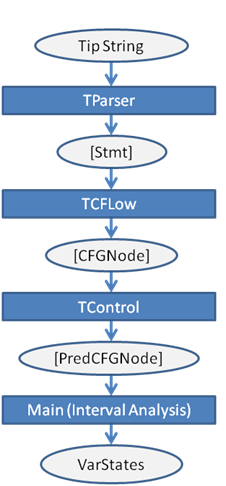
\includegraphics[width=0.3\linewidth]{grafico}}
% \caption{Tip Program Transformation}
% \label{fig:hskia}
% \end{figure}


\section{User Guide}
To use the program a compilation thru \emph{ghc} is required, the procedure is as follow:
\begin{verbatim}
$ ghc --make Main.hs -o hskia
\end{verbatim}

The previous step should generate a \emph{hskia} executable file,
\begin{verbatim}
$ ./hskia 
Usage: hskia [-i -p -a -o] filename

      -a: get the production list from file

      -p: get the predecesors list from file

      -i: start the interval analysis
      
      -o: optimize the code given in filename 
\end{verbatim}

\ldots where:
\begin{description}
  \item[-a] Prints the productions for the tip program in filename, this does not include the interval analysis.
  \item[-p] Prints the predecesors list for debugging the program analysis later, this option also does not include the interval analysis. 
  \item[-i] Starts the interval analysis, including widening and generates the analysis report.
  \item[-o] Creates an optimized version of the tip program <filename>, it includes the interval analysis 
\end{description}

\bibliographystyle{apacite}
\begin{thebibliography}{XXX}
  \bibitem{Schwartzbach} Schwartzbach, I. , Lecture Notes on Static Analysis. University of Aarthus, Denmark. mis\@bricks.dk.

  \bibitem{Bourdoncle} Bourdoncle, F. (1993, January). Efficient chaotic iteration strategies with widenings. In Formal Methods in Programming and their Applications (pp. 128-141). Springer Berlin Heidelberg.

  \bibitem{Cousot} Cousot, P., \& Cousot, R. (1977, January). Abstract interpretation: a unified lattice model for static analysis of programs by construction or approximation of fixpoints. In Proceedings of the 4th ACM SIGACT-SIGPLAN symposium on Principles of programming languages (pp. 238-252). ACM.

\end{thebibliography}


\end{document}
